% Vorlesung 31.10.18
 
\chapter{Geometrische Optik}

\section{Lichtstrahlen}

Licht hat eine \textbf{Ausbreitungsgeschwindigkeit} $ s = ct $. Diese Geschwindigkeit ist nur im Vakuum konstant und hängt von der Materie die der Lichtstrahl durchläuft ab. Diese Geschwindigkeit im Medium ist gegeben durch den \textbf{Brechungsindex}.
\begin{equation*}
\rmbox{n = \frac{c_{\tx{Vakuum}}}{c_{\tx{Medium}}}} \qquad \qquad \begin{array}{ll}
\tx{Luft:} & n = 1{,}00027 \\
\tx{Wasser:} & n = 1{,}333 \\
\tx{Diamant:} & n = 2{,}417
\end{array}
\end{equation*}
\lcom{Warum ist das denn so? Wie interagieren die elektromagnetischen Felder des Lichstrahls also mit der Materie?}\\
Antwort:\\
\lcom{Die Ladungsträger in der Materie erfahren aufgrund der elektrischen Felder eine Kraft. Die Ströme der bewegten Ladungen Wechselwirkungen mit den Magnetischen Feldern, jedoch ist dieser Effekt viel kleiner als der der $ \vec{E} $-Felder.\\
Die Elektronen kann man sich mit einer Feder an der Atomkern gebunden Vorstellen. Mit dem $ \vec{E} $-Feld des Lichtstrahls haben wir das Modell eines getriebenen gedämpften harmonischen Oszillators: \textbf{Das Lorenz-Lorentz-Oszillator Modell}.}\\
Genaugenommen kann man sich das auch so Vorstellen, dass die Photonen immer wieder absorbiert und nach einer Zeitverzögerung abgestrahlt werden, jedoch ist dies schwer zu berechnen.\\[10pt]
\emph{Bemerkung:}\\
zwei Medien $ n_1 > n_2 $\\
$ n_1 $: \textbf{optisch dichter}\\
$ n_2 $: \textbf{optisch dünner}

\section{Das Fermat'sche Prinzip}

\subsection{Fermat'sches Prinzip}

\begin{minipage}{.6\linewidth}
	Die Ausbreitung des Lichts zwischen zwei Punkten erfolgt auf dem Weg, für den die benötigte Zeit extremal ist.
\end{minipage}%
\begin{minipage}{.4\linewidth}
	%t1:
	\centering
	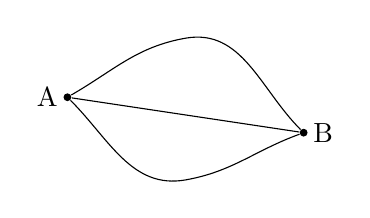
\begin{tikzpicture}[scale=1.5]
	\node[circle,fill=black,inner sep=1pt, minimum size=1pt] at (0,0) (A) {};
	\node[circle,fill=black,inner sep=1pt, minimum size=1pt] at (2,-.3) (B) {};
	\node[left] at (A) {A};
	\node[right] at (B) {B};
	\draw (A) to[out=30,in=190] (1,.5) to[out=10,in=135] (B);
	\draw (A) to[out=-45,in=190] (1,-.7) to[out=10,in=200] (B);
	\draw (A) -- (B);
	\end{tikzpicture}
\end{minipage}%
\\
$ \Rightarrow $ Konsequenz $\rmbox{\tx{Der Stahlengang ist umkehrbar \mau}}$

\subsubsection{Mathematische Handwerkzeuge}

\begin{equation*}
t = \frac{1}{c_{\tx{Vakuum}}} \int_{P_1}^{P_2} n(s) ds
\end{equation*}
Parametrisierung des Wegs $ \tau $
\begin{equation*}
\vec{x} = \vec{x} (\tau)
\end{equation*}
\begin{equation*}
t(\vec{x}) = \frac{1}{c_{\tx{Vakuum}}} \int_{P_1}^{P_2} n(\vec{x(\tau)}) \sqrt{\left(\frac{\dd\vec{x}}{\dd\tau}\right)^2} d\tau
\end{equation*}

\subsection{Weg zwischen zwei Punkten A und B}

%t2:
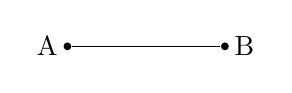
\begin{tikzpicture}
	\node[circle,fill=black,inner sep=1pt, minimum size=1pt] at (0,0) (A) {};
	\node[circle,fill=black,inner sep=1pt, minimum size=1pt] at (2,0) (B) {};
	\node[left] at (A) {A};
	\node[right] at (B) {B};
	\draw (A) -- (B);
\end{tikzpicture}

\subsection{Reflexionsgesetz}

\begin{minipage}{.6\linewidth}
	\folie{zu Reflexion an Oberflächen}\\
	Berechnung der Wegstrecke
	\begin{equation*}
	s(x) = \sqrt{a^2 + x^2} + \sqrt{d^2 + (b-x)^2}
	\end{equation*}
\end{minipage}%
\begin{minipage}{.4\linewidth}
	%t3:  % folie:
	\centering
	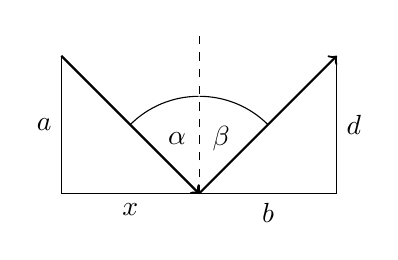
\begin{tikzpicture}[scale=1.75]
	\node at (0,0) (m) {};
	\node at (-1,0) (l) {};
	\node at (1,0) (r) {};
	\node at (0,1) (mu) {};
	\node at (-1,1) (lu) {};
	\node at (1,1) (ru) {};
	\draw[thick,->] (-1,1) -- (0,0);
	\draw[thick,->] (0,0) -- (1,1);
	\draw (-1,1) -- (-1,0) -- (0,0) -- (1,0) -- (1,1);
	\draw[dashed] (0,0) -- (0,1.2);
	\draw (.5,.5) arc (45:90:20pt);
	\draw (-.5,.5) arc (135:90:20pt);
	\node at (.16,.4) () {$ \beta $};
	\node at (-.16,.4) () {$ \alpha $};
	\node[below] at (-.5,0) {$ x $};
	\node[below] at (.5,0) {$ b $};
	\node[right] at (1,.5) {$ d $};
	\node[left] at (-1,.5) {$ a $};
	\end{tikzpicture}
\end{minipage}%
\\
Extremum:\\
\lcom{Da wir und in einem homogenen Medium befinden und die Lichtgeschwindigkeit konstant ist, ist die Strecke $ s $ proportional zur Zeit $ t $ und wir können das Extremum der Strecke berechnen.}
\begin{equation*}
\frac{\dd s}{\dd x} = 0
\end{equation*}
\begin{equation*}
\Rightarrow \ub{\frac{x}{\sqrt{a^2 + x^2}}}_{\sin \alpha} = \ub{\frac{b-x}{\sqrt{d^2 + (b-x)^2}}}_{\sin \beta}
\end{equation*}
\begin{minipage}{.2\linewidth}
	$ \phantom{M} $
\end{minipage}
\begin{minipage}{.6\linewidth}
	\frbox{Reflexionsgesetz}{\begin{equation*}
		\sin \alpha = \sin \beta
		\end{equation*}}
\end{minipage}\\[5pt]
\lcom{Einfallswinkel gleich Ausfallswinkel.}

\subsection{Brechungsgesetz von Snellius}

\begin{equation*}
n_1 \neq n_2 \qquad \Leftrightarrow \qquad n(s) \neq \const
\end{equation*}
\begin{minipage}{\linewidth}
	%t4:
	\centering
	\begin{tikzpicture}[scale=1.5]
	\draw[draw=none,fill=gray!10] (-1.5,0) rectangle (1.5,-1.1);
	\node[circle,fill=black,inner sep=1pt, minimum size=1pt] at (-.75,.4) (A) {};
	\node[circle,fill=black,inner sep=1pt, minimum size=1pt] at (1,-.75) (B) {};
	\node[anchor=south east] at (A) {A};
	\node[anchor=north west] at (B) {B};
	\node[circle,fill=black,inner sep=1pt, minimum size=1pt] at (-.5,0) (a) {};
	\node[circle,fill=black,inner sep=1pt, minimum size=1pt] at (.5,0) (b) {};
	\node[circle,fill=black,inner sep=1pt, minimum size=1pt] at (-.9,0) (c) {};
	\draw[thick] (A) -- (b) -- (B) -- (a) -- (A);
	\draw[thick] (A) -- (c) -- (B);
	\draw (-1.5,0) -- (1.5,0);
	\filldraw[draw=none,pattern=north east lines] (-1.5,0) rectangle (1.5,-.1);
	\node at (-2,.5) {$ c_1 n_1 $};
	\node at (-2,-.5) {$ c_2 n_2 $};
	\draw[dashed] (0,-1) -- (0,1);
	\end{tikzpicture} \hspace{80pt}
	\begin{tikzpicture}[scale=1.5]
	\draw[draw=none,fill=gray!10] (-1.5,0) rectangle (1.5,-1.1);
	\filldraw[draw=none,pattern=north east lines] (-1.5,0) rectangle (1.5,-.1);
	\node[circle,fill=black,inner sep=1pt, minimum size=1pt] at (-1,.75) (A) {};
	\node[circle,fill=black,inner sep=1pt, minimum size=1pt] at (1,-.75) (B) {};
	\node[anchor=south east] at (A) {A};
	\node[anchor=north west] at (B) {B};
	\node[circle,fill=black,inner sep=1pt, minimum size=1pt] at (-.5,0) (a) {};
	\node[circle,fill=black,inner sep=1pt, minimum size=1pt] at (.5,0) (b) {};
	\draw[thick] (A) -- (b) -- (B) -- (a) -- (A);
	\draw[thick] (-1.5,0) -- (1.5,0);
	\draw[thick,dashed] (A) -- (-1,0);
	\draw[dashed] (0,-1) -- (0,1);
	\draw[very thick,->] (-1,0) -- (b) node[anchor=south west] {$ x $};
	\end{tikzpicture} \hspace{30pt}
\end{minipage}%
\\[10pt]
\noindent
Berechnung des Laufzeit des Lichts
\begin{equation*}
t(x) = \frac{\sqrt{x^2 + a^2}}{c_1} + \frac{\sqrt{(b-x)^2 + d^2}}{c_2} = \frac{1}{c} \left(n_1 \sqrt{x^2 + a^2} + n_2 \sqrt{(b-x)^2 + d^2}\right)
\end{equation*}
\folie{zu Brechung}
$ \frac{dt}{dx} = 0 $\\
\begin{minipage}{.55\linewidth}
	\frbox{Brechungsgesetz}{\begin{equation*}
		\Rightarrow n_1 \sin \alpha = n_2 \sin \beta
		\end{equation*}}
\end{minipage}%
\begin{minipage}{.45\linewidth}
	%t5:
	\centering
	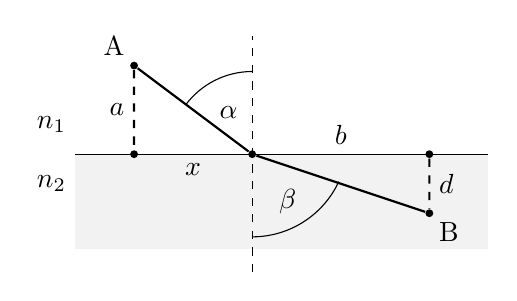
\begin{tikzpicture}[scale=1.5]
	\draw[draw=none,fill=gray!10] (-1.5,0) rectangle (2,-.8);
	\node[circle,fill=black,inner sep=1pt, minimum size=1pt] at (-1,.75) (A) {};
	\node[circle,fill=black,inner sep=1pt, minimum size=1pt] at (1.5,-.5) (B) {};
	\node[anchor=south east] at (A) {A};
	\node[anchor=north west] at (B) {B};
	\node[circle,fill=black,inner sep=1pt, minimum size=1pt] at (-1,0) (a) {};
	\node[circle,fill=black,inner sep=1pt, minimum size=1pt] at (1.5,0) (b) {};
	\node[circle,fill=black,inner sep=1pt, minimum size=1pt] at (0,0) (o) {};
	\draw[thick] (A) -- (o) -- (B);
	\draw[thick,dashed] (b) -- (B);
	\draw (-1.5,0) -- (2,0);
	\draw[thick,dashed] (A) -- (-1,0);
	\draw[dashed] (0,-1) -- (0,1);
	\draw (0,-.7) arc (-90:-25:23pt);
	\draw (0,.7) arc (90:143.5:20pt);
	\node at (-.2,.35) {$ \alpha $};
	\node at (.3,-.4) {$ \beta $};
	\node[left] at (-1,.375) {$ a $};
	\node[below] at (-.5,0) {$ x $};
	\node[above] at (.75,0) {$ b $};
	\node[right] at (1.5,-.25) {$ d $};
	\node at (-1.7,-.25) {$ n_2 $};
	\node at (-1.7,.25) {$ n_1 $};
\end{tikzpicture}
\end{minipage}%

\section{Einfache Anwendungen}

\subsection{Totalreflexion}

$ \rightarrow $ siehe Experimentalphysik II\\
\folie{zur Totalreflexion z.B. unter Wasser}
\begin{equation*}
\sin\alpha_{\tx{TR}} = \frac{n_2}{n_1}
\end{equation*}

\subsection{Optisches Prisma}

\lcom{Bei Drehung des Prismas kann der Winkel $ \delta $ verändert werden. Hier gibt es es ein Minimum, jedoch kann er nie null werden, da das Licht nie gerade durch das Prisma hindurch kommen kann.}

\subsubsection{Beobachtung I}

\begin{minipage}{.55\linewidth}
	Die Ablenkung ist minimal für den symmetrischen  Strahlengang
	\begin{equation*}
	\sin \frac{\delta_{\tx{min}} + \gamma}{2} = n \sin \frac{\gamma}{2}
	\end{equation*}
	\folie{Demtröder: Prisma}
	\vspace{40pt}
\end{minipage}%
\begin{minipage}{.45\linewidth}
	%t6:
	\centering
	\begin{tikzpicture}
		\draw[fill=gray!10] (2,0) -- ++(120:4cm) -- ++(240:4cm) -- ++(360:4cm);
		\coordinate (d) at ($(60:2cm) + (120:2cm)$);
		\coordinate (a) at (120:2cm); %($ (-2,0)!.4!(d) $);
		\coordinate (c) at (60:2cm);
		\coordinate (b) at ($ (2,0)!.6!(d) $) {};
		\draw[dashed] ($(a) + (150:1cm)$) -- ++(-30:2cm);
		\draw[dashed] ($(b) + (30:1cm)$) -- ++(210:2cm);
		\draw[thick] (3,1.5) -- (b) -- (a) -- ++(220:2cm);
		\draw[dashed] (a) -- ++(40:4cm);
		\centerarc[](a)(150:220:.8cm);
		\node[left,xshift=-5pt,yshift=-2pt] at (a) {$ \alpha_1 $};
		\centerarc[](a)(-30:10:.8cm);
		\node[anchor=north west,yshift=-4pt] at (a) {$ \beta_1 $};
		\centerarc[](b)(190:210:.8cm);
		\node[anchor=north east,yshift=-5pt] at (b) {$ \beta_2 $};
		\centerarc[](b)(30:-14:.9cm);
		\node[right,xshift=8pt,yshift=1pt] at (b) {$ \alpha_2 $};
		\coordinate (o) at (-.26,2.34) {};
		\centerarc[](o)(40:-14:2.5cm);
		\node at ($ (b) + (1.7,.8) $) {$ \delta $};
		\centerarc[](d)(-120:-60:.6cm);
		\node[below,yshift=-3pt] at (d) {$ \gamma $};
		\node[above] at (-1,0) {$ n = n_2 $};
		\node[below] at (-1.5,-.3) {$ n = n_1 $};
	\end{tikzpicture}
\end{minipage}%
\\
\textbf{Berechnung:}
\begin{enumerate}[(i)]
	\item $ \gamma = \beta_1 + \beta_2 $
	\item $ \delta = \alpha_1 - \beta_1 + \alpha_2 - \beta_2 $
	\item $ \sin \alpha_1 = n \sin \beta_1 \quad , \quad \sin \alpha_2 = n \sin \beta_2 $
\end{enumerate}
gesucht ist $ \frac{d\delta}{d \alpha_1} = 0 $\\
$ \Rightarrow $
\begin{enumerate}[(i)]
	\item $ \tx{d}\gamma = \tx{d}\beta_1 + \tx{d}\beta_2 = 0 $
	\item $ \tx{d}\alpha_1 = \tx{d}\alpha_2 \qquad (\delta = \alpha + \alpha - \gamma) \qquad (\mathrm{d} \delta = 0) $
	\item $ \cos \alpha_1 \tx{d} \alpha_1 = n \cos \beta_1 \tx{d} \beta_1 $\\
	$ \cos \alpha_1 \tx{d} \alpha_2 = n \cos \beta_2 \tx{d} \beta_2 $
\end{enumerate}

$$\Rightarrow\frac{\cos\alpha_1\cancel{\tx{d}\alpha_1}}{\cos\alpha_2\cancel{\tx{d}\alpha_2}}=\frac{\cos\beta_1\cancel{\tx{d}\beta_1}}{\cos\beta_1\cancel{\tx{d}\beta_2}}$$
$$\Rightarrow\frac{1-\sin^2\alpha_1}{1-\sin^2\alpha_2}=\frac{1-\sin^2\beta  a_1}{1-\sin^2\beta_2}=\frac{n^2-\sin^2\alpha_1}{n^2-\sin^2\alpha_2}$$\\[-10pt]
$$\left.\begin{array}{c}
\alpha_1=\alpha_2 \\
\beta_1=\beta_2\end{array} \right\} \textrm{ symmetrischer Strahlengang}$$\\
\noindent
$ \Rightarrow \quad \delta_{\tx{min}} = \alpha_1 + \alpha_2 - \gamma = 2 \alpha - \gamma \qquad \gamma = 2 \beta $
\begin{equation*}
\Rightarrow \quad \sin \alpha = n \sin \beta \quad \Rightarrow \quad \rmbox{\sin \frac{\delta_{\tx{min}} + \gamma}{2} = n \sin \frac{\gamma}{2}}
\end{equation*}
\begin{flushright}
	$ \square $
\end{flushright}
\emph{Bemerkung:}\\
Dieser Zusammenhang wurde früher zur Bestimmung von $ n $ genutzt \mau\\
\lcom{*Professor redet darüber, dass wir immer kompliziertere Experimente verstehen können, und diese aufgrund des Aufwands bei der Ausführung nicht mehr immer in der Vorlesung gezeigt werden können. Wir sollen lernen uns Experimente vorzustellen ohne sie direkt zu sehen und die Formeln als Handlungsanweisungen zu sehen die wir nutzen können. Abgesehen davon sollen wir uns auch im klaren darüber sein wie genau verschiedene Messmethoden sind.*}

\subsubsection{Beobachtung II}

optische Dispersion:
\begin{equation*}
\frac{\dd n(\lambda)}{\dd\lambda} < 0 \qquad (\tx{normale Dispersion})
\end{equation*}
(Bei der anormalen Dispersion ist $ \frac{\dd n(\lambda)}{\dd\lambda} > 0 $)\\
\folie{zur Dispersion: Beispiel Regenbogen}\\[5pt]
\lcom{Wieso gibt es Dispersion? Vorstellung: Die Atome mit ihren Elektronen haben Resonanzfrequenzen. Somit ist die erzwungene Schwingung, die die Licht-Welle in der Materie anregt, von der Frequenz des Lichts abhängig.\\
Die meisten Resonanzfrequenzen liegen im Ultravioletten-Bereich. Deshalb sehen wir meist normale Dispersion. Im Bereich über Ultraviolettem Licht ist auch anormale Dispersion beobachtbar.}\\[5pt]
$ \Rightarrow $ Experimentalphysik II
%\lcom{*Das geht wirklich nicht! Was soll man denn da machen? Das ist echt lässtig!*}

\section{Sphärische, dünne Linse}

\lcom{Zunächst einmal betrachten wir sphärische Linsen speziell dünne Linsen: Wir betrachten die dünne Linse als eine unendlich-dünne Linse, da wir hierbei einige vereinfachungen machen können (Taylor-entwicklungs-Terme fallen weg).}

\subsection{Brennpunkt und Brennebene}

\folie{zur Sammel- und Streulinsen}\\
Wir betrachten zunächst den Strahlengang einer Linse:\\
\rbox{\begin{minipage}{\linewidth}
		\lcom{Lieblingsprüfungsfrage: Parallel einfallendes Licht, das nicht parallel zur optischen Achse verläuft, in eine Sammellinse. Strahlen werden immer noch fokussiert aber Brennpunkt verschoben. Konstruktion mit Zentralstrahlengang \mau}
	\end{minipage}}
\noindent
\folie{zur der Lieblingsfrage}

\subsubsection{3 Regeln zur Konstruktion von Strahlengängen}

Nur für dünne Linsen:
\begin{enumerate}[1)]
	\item Parallel einfallende Strahlen fallen durch den Brennpunkt aus
	\item Durch Brennpunkt einfallender Strahlen fallen parallel aus
	\item Der Zentralstrahl wird nicht abgelenkt
\end{enumerate}

\subsection{Berechnung des Brennpunktes bzw. der Brennweite}

\lcom{Bei der Streulinse genau dasselbe nur ein negatives Vorzeichen an der Brennweite.}\\
\folie{zu Strahlengängen durch Sammellinsen}\\[5pt]
Ein Linsenstück im Abstand $ h $ von der optischen Achse betrachten wir als Prisma.\\[5pt]
Näherungen der ,,dünnen`` Linse\\[5pt]
alle Winkel sind klein $ \rightarrow $ trigonometrische Näherungen\\
$ \sin(x) \approx x \qquad \cos(x) \approx 1 \qquad \tan(x) \approx x $\\[5pt]
\textbf{Berechnung:}\\
Ablenkung des Strahls\\
\begin{minipage}{.4\linewidth}
	\begin{enumerate}
		\item[(i)] $ \delta = \alpha_1 - \beta_1 + \alpha_2 - \beta_2 $
		\item[(ii)] $ \beta_1 + \beta_2 = \gamma $
		\item[(iii)] $ n_1 \alpha_1 \approx n_2 \beta_1 \qquad n_2 \beta_2 \approx n_1 \alpha_2 $
		\begin{equation*}
		\Rightarrow \quad \delta = \gamma\left(\frac{n_2}{n_1} - 1\right)
		\end{equation*}
	\end{enumerate}
\end{minipage}%
\begin{minipage}{.6\linewidth}
	%t8:
	\centering
	\begin{tikzpicture}
		\draw[dashed] (0,4) arc (150:170:400pt);
		\draw[dashed] (0,4) arc (30:10:400pt);
		\centerarc[](0,4)(-118:-62:.8cm);
		\node[below,yshift=-7pt] at (0,4) {$ \gamma $};
		%\node[circle,fill=black,inner sep=1pt,minimum size=1pt] at (1.55,0) {};
		%\node[circle,fill=black,inner sep=1pt,minimum size=1pt] at (.95,2) {};
		\coordinate (x) at (1.55,0);
		\coordinate (x2) at (-1.55,0);
		\coordinate (y) at (.95,2);
		\coordinate (y2) at (-.95,2);
		\draw[fill=gray!10] (x) -- (y) -- (y2) -- (x2) -- (x);
		\coordinate (b) at ($ (x)!.6!(y) $);
		\coordinate (a) at ($ (x2)!.4!(y2) $);
		%\draw(a) -- (b);
		% winkel der seiten ist 107 grad bzw 73 grad
		\draw[dashed] ($(a) + (163:1cm)$) -- ++(-17:2cm);
		\draw[dashed] ($(b) + (197:1cm)$) -- ++(17:2.75cm);
		\draw[thick] (3,.5) -- (b) -- (a) -- ++(220:2.5cm);
		\draw[dashed] (a) -- ++(40:5cm);
		\centerarc[](a)(163:220:.8cm);
		\node[left,xshift=-5pt,yshift=-2pt] at (a) {$ \alpha_1 $};
		\centerarc[](a)(-17:10:.8cm);
		\node[anchor=north west,yshift=-4pt] at (a) {$ \beta_1 $};
		\centerarc[](b)(190:197:.8cm);
		\node[anchor=north east,yshift=-5pt] at (b) {$ \beta_2 $};
		\centerarc[](b)(17:-20:.9cm);
		\node[right,xshift=8pt,yshift=-1pt] at (b) {$ \alpha_2 $};
		\centerarc[](b)(17:-20:1.5cm);
		\node[right,xshift=25pt,yshift=2pt] at (b) {$ \delta_2 $};
		\centerarc[](a)(40:12:4.02cm);
		\node[right,xshift=87pt,yshift=45pt] at (a) {$ \delta_1 $};
		\coordinate (o) at (-.22,1.71) {};
		%\node[circle,fill=black,inner sep=1pt,minimum size=1pt] at (-.22,1.71) {};
		%\draw (b) -- ++(160:3cm);
		\centerarc[](o)(40:-20:3.4cm);
		\node at ($ (b) + (2.2,1) $) {$ \delta $};
		\node[above] at (1,0) {$ n_2 $};
		\node[below] at (1.2,-.3) {$ n_1 $};
	\end{tikzpicture}
\end{minipage}%
\\
Winkel $ \gamma $:\\[10pt]
\begin{minipage}{.4\linewidth}
	\begin{enumerate}
		\item[(iv)] $ \gamma = \gamma_1 + \gamma_2 $
		\item[(v)] $ \gamma_1 \approx \frac{h}{R_1} \quad ;\quad \gamma_2 \approx \frac{h}{R_2} $
		\begin{equation*}
		\Rightarrow \qquad \gamma = h \left(\frac{1}{R_1} - \frac{1}{R_2}\right)
		\end{equation*}
	\end{enumerate}
\end{minipage}%
\begin{minipage}{.6\linewidth}
	%t9:
	\centering
	\begin{tikzpicture}[decoration=brace,scale=.8]
		\coordinate (a) at ( .25,0) {};
		\coordinate (b) at (-.25,0) {};
		\draw[fill=gray!10,draw=none] ($(b)+(135:2cm) + (-0.02,0)$) rectangle ($(a)+(-28:3cm)$);
		\node[circle,fill=black,inner sep=1pt,minimum size=1pt] at (a) {};
		\node[circle,fill=black,inner sep=1pt,minimum size=1pt] at (b) {};
		\centerarc[thick,fill=gray!10](a)(-28:28:3cm);
		\centerarc[thick,fill=gray!10](b)(135:225:2cm);
		\draw[dashed] (-3,0) -- (4,0);
		\draw (a) -- ++(19:3cm);
		\draw (b) -- ++(150:2cm);
		\draw[color=gray!70] ($(b)+(135:2cm)$) -- ($(a)+(28:3cm)$);
		\draw[color=gray!70] ($(b)+(225:2cm)$) -- ($(a)+(-28:3cm)$);
		\draw[red] (-2.5,0) -- (-2.5,1);
		\draw[red] (-2.6,1) -- (-2.4,1);
		\draw[red,dashed] (-2.5,1) -- (-2,1);
		\draw[decorate, xshift=-4pt,red]  (-2.5,0) -- node[left=0.4pt] {$h$}  (-2.5,1);
		\node[below] at (-1.25,0) {$ R_1 $};
		\node[below] at (1.8,0) {$ R_2 $};
		\centerarc[](b)(180:150:1.2cm);
		\centerarc[](a)(0:19:1.5cm);
		\node[right,yshift=4pt,xshift=17pt] at (a) {$ \gamma_2 $};
		\node[left,yshift=4pt,xshift=-10pt] at (b) {$ \gamma_1 $};
	\end{tikzpicture}
\end{minipage}%
\\
Winkel $ \delta $:\\[10pt]
\begin{minipage}{.4\linewidth}
	\begin{enumerate}
		\item[(vi)] $ \delta \approx \frac{h}{f} $
	\end{enumerate}
\end{minipage}%
\begin{minipage}{.6\linewidth}
	%t10:
	\centering
	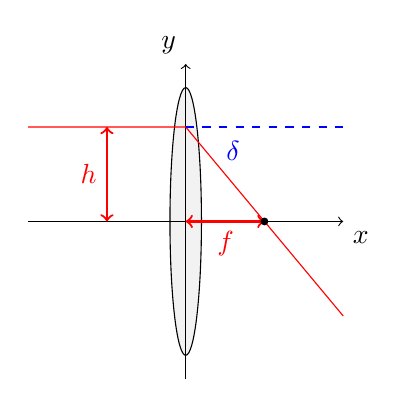
\begin{tikzpicture}
		\draw[fill=gray!10] (0,0) ellipse (.2cm and 1.7cm);
		\draw[->] (-2,0) -- (2,0) node[anchor=north west] {$ x $};
		\draw[->] (0,-2) -- (0,2) node[anchor=south east] {$ y $};
		\draw[red] (-2,1.2) -- (0,1.2) -- (2,-1.2);
		\draw[red,thick,<->] (0,0) -- (1,0) node[below,xshift=-14pt] {$ f $};
		\draw[red,thick,<->] (-1,0) -- (-1,1.2) node[left,yshift=-17pt] {$ h $};
		\node[circle,fill=black,inner sep=1pt,minimum size=1pt] at (1,0) {};
		\draw[blue,dashed] (0,1.2) -- (2,1.2);
		\centerarc[blue](0,1.2)(0:-50:1cm);
		\node[blue] at (.6,.9) {$ \delta $};
	\end{tikzpicture}
\end{minipage}%

% 6.11.18 Vorlesung 7

\frbox{Linsenschleiferformel}{\begin{equation*}
\Rightarrow \quad \frac{1}{f} = \frac{n_2 - n_1}{n_1} \left(\frac{1}{R_1} - \frac{1}{R_2}\right)
\end{equation*}}

\noindent
$ \Rightarrow $ Die Brennweite $ f $ ist unabhängig von $ h $. \lcom{Hätte wir oben keine Näherungen für die Winkelfunktionen benutzt (bei allen Rundungssymbolen), dann wäre die Brennweite abhängig von der Höhe $ h $. Hier sehen wir, dass die Gleichung für eine dünne Linse nur eine Annäherung an echte Linsen ist.}\\[10pt]
\textbf{Def: Brechkraft}
\begin{equation*}
D = \frac{n}{f}
\end{equation*}
\emph{Bemerkung:}\\
$ D = D_{\tx{Vorne}} + D_{\tx{Hinten}} $

\subsection{Abbildung (am Beispiel einer Sammellinse)}

\begin{minipage}{.5\linewidth}
	Berechnung:
	\begin{enumerate}[i)]
		\item $ \delta = \alpha + \beta $
		\item $ \alpha \approx \frac{h}{a} \quad \beta \approx \frac{h}{b} $
		\item $ \delta \approx \frac{h}{f} $
	\end{enumerate}
\end{minipage}%
\begin{minipage}{.5\linewidth}
	%t1:
	\centering
	\begin{tikzpicture}
		\draw[fill=gray!10] (0,0) ellipse (.2cm and 1.7cm);
		\draw[dashed]  (0,-2) -- (0,2);
		\draw (-3,0) -- (3,0);
		\coordinate (A) at (-2.5,0);
		\coordinate (B) at (2.5,0);
		\node[below] at (A) {$ A $};
		\node[below] at (B) {$ B $};
		\draw[thick] ($ (A) + (0,-.1) $) -- ++(0,.2);
		\draw[thick] ($ (B) + (0,-.1) $) -- ++(0,.2);
		\coordinate (M) at (0,1);
		\draw (A) -- (M) -- (B);
		\node[below] at ($ (0,0)!.5!(A) $) {$ a $};
		\node[below] at ($ (0,0)!.5!(B) $) {$ b $};
		\draw[dashed,thick] (M) -- ++($ (B) + (M) $);
		\centerarc[](M)(22:-22:1cm);
		\node[right,xshift=10pt] at (M) {$ \delta $};
		\centerarc[](A)(22:0:1.5cm);
		\node[right,xshift=20pt,yshift=5pt] at (A) {$ \alpha $};
		\centerarc[](B)(158:180:1.5cm);
		\node[left,xshift=-25pt,yshift=6pt] at (B) {$ \beta $};
		\draw (A) -- ++(-158:1cm);
		\draw (B) -- ++(-22:1cm);
	\end{tikzpicture}
\end{minipage}%

\noindent
\frbox{Abbildungsgesetz}{
\begin{equation*}
\Rightarrow \frac{1}{f} = \frac{1}{a} + \frac{1}{b}
\end{equation*}}
\textbf{Abbildung eines Gegenstands $ G $:}\\
Graphisch:
\begin{enumerate}[(1)]
	\item parallel ein $ \rightarrow $ durch Brennpunkt aus
	\item durch Brennpunkt ein $ \rightarrow $ parallel aus
	\item Zentralstrahl läuft gerade
\end{enumerate}
\begin{minipage}{.5\linewidth}
	\textbf{Rechnerisch}
	\begin{enumerate}[(i)]
		\item $ \frac{1}{f} = \frac{1}{a} + \frac{1}{b} $
		\item $ \frac{A}{a} = \frac{B}{b} $
	\end{enumerate}
\end{minipage}%
\begin{minipage}{.5\linewidth}
	%t2:
	\centering
	\begin{tikzpicture}
		\draw[fill=gray!10] (0,0) ellipse (.2cm and 1.7cm);
		\draw[dashed]  (0,-2) -- (0,2);
		\draw (-3,0) -- (3,0);
		\coordinate (A) at (-2.5,1);
		\coordinate (B) at (2.5,-1);
		\node[above] at (A) {$ A $};
		\node[below] at (B) {$ B $};
		\draw[thick] ($ (-2.5,0) + (0,-.1) $) -- ++(0,.2);
		\draw[thick] ($ (2.5,0) + (0,-.1) $) -- ++(0,.2);
		\coordinate (M) at (0,1);
		\coordinate (m) at (0,-1);
		\draw (A) -- (M) -- (B);
		\draw (A) -- (B);
		\draw (A) -- (m) -- (B);
		\node[below] at ($ (0,0)!.5!(-2.5,0) $) {$ f $};
		\node[above] at ($ (0,0)!.5!(2.5,0) $) {$ f $};
		\draw[thick] ($ (1.25,0) + (45:.1) $) -- ++(-135:.2);
		\draw[thick] ($ (1.25,0) + (-45:.1) $) -- ++(135:.2);
		\draw[thick] ($ (-1.25,0) + (45:.1) $) -- ++(-135:.2);
		\draw[thick] ($ (-1.25,0) + (-45:.1) $) -- ++(135:.2);
		\node[below] at (-2,0) {$ a $};
		\node[below] at (2,0) {$ b $};
		\draw[very thick,->] (-2.5,0) -- (A);
		\draw[very thick,->] (2.5,0) -- (B);
		\node[circle,draw=black,inner sep=1pt] at (-1,1.5) {1};
		\node[circle,draw=black,inner sep=1pt] at (-.6,.7) {2};
		\node[circle,draw=black,inner sep=1pt] at (-.7,-1) {3};
	\end{tikzpicture}
\end{minipage}%

\section{Abbildungsfehler}

$ \Rightarrow $ Beschränkung durch Beschreibung mit geometrischer Optik\\
$ \Rightarrow $ Näherungen (dünne Linse)

\subsection{Dicke Linsen}

\folie{Dicke Linsen}\\
Brechung der Lichtstrahlen an zwei Hauptebenen
%
%
%
% Bilder von Volie Dicke Linsen einfügen
%
%
%
\subsection{Sphärische Abberation}

\folie{Sphärische Abberation}

\subsection{Chromatische Abbreration}

\folie{Chromatische Abberation}\\
optische Dispersion

\subsection{Astigmatismus}

\folie{Astigmatismus}

\subsection{Absorption}

Bei verunreinigten Stoffen wird Licht absorbiert.

\subsection{Beugung}

\lcom{Werden wir später behandeln.}

\subsection{Optisches Auflösungsvermögen}

\rbox{Mit freilaufenden Wellen lassen sich keine Strukturen auflösen, die deutlich kleiner sind als die Wellenlänge $ \lambda $ sind.}

\section{Optische Instrumente}

\subsection{Vergrößerung}

\textbf{Sehwinkel:}
%t3:
\hspace{40pt}
\begin{tikzpicture}
	\draw ($ (-.5,0) + (25:.7cm) $) -- ++(-155:.7cm) -- ++(-25:.7cm);
	\centerarc[](-.5,0)(-25:25:.5cm);
	\draw (3,0) -- (0,0) -- (3,1);
	\draw[thick,->] (3,0) -- (3,1) node[right,yshift=-15pt] {$ G $};
	\centerarc[](0,0)(0:18.5:1.5cm);
	\node[yshift=5pt,xshift=30pt] at (0,0) {$ \alpha $};
\end{tikzpicture}

\begin{equation*}
\tan\alpha = \frac{\tx{Größe des Objekts}}{\tx{Entfernung des Objekts}}
\end{equation*}
\textbf{Winkelvergrößerung}
\begin{equation*}
V = \frac{\tx{Sehwinkel mit Instrument}}{\tx{Sehwinkel ohne Instrument}}
\end{equation*}
\textbf{Lateralvergrößerung oder Abbildungsmaßstab}
\begin{equation*}
L = \frac{\tx{Bildgröße}}{\tx{Gegenstandsgröße}}
\end{equation*}

\subsection{Das menschliche Auge}

\folie{menschliches Auge}\\
Hornhaut \& Linse. Die Hornhaut hat den größten Beitrag zur Brechung\\[5pt]
\textbf{Definition: Brennweite der deutlichen Sehweite}
\begin{equation*}
25 \, \tx{cm}
\end{equation*}
\begin{equation*}
\Rightarrow \quad \tan \alpha_{\tx{Auge}} = \frac{G}{25 \, \tx{cm}}
\end{equation*}
Vergrößerung
\begin{equation*}
V = \frac{\tx{Sehwinkel mit Instrument}}{\alpha_{\tx{Auge}}} = (\tx{Sehwinkel mit Instrument}) \frac{25 \, \tx{cm}}{G}
\end{equation*}

\subsection{Optisches Instrument mit einer Linse: Lupe}

%t4:
\begin{center}
\begin{tikzpicture}
	\draw[fill=gray!10] (0,0) ellipse (.2cm and 1.7cm);
	\draw[dashed] (0,-2) -- (0,2);
	\draw (-4,0) -- (3,0);
	\node[below] at ($ (0,0)!.5!(-3.6,0) $) {$ f $};
	\node[above] at ($ (0,0)!.5!(3.6,0) $) {$ f $};
	\draw[thick] ($ (1.8,0) + (45:.1) $) -- ++(-135:.2);
	\draw[thick] ($ (1.8,0) + (-45:.1) $) -- ++(135:.2);
	\draw[thick] ($ (-1.8,0) + (45:.1) $) -- ++(-135:.2);
	\draw[thick] ($ (-1.8,0) + (-45:.1) $) -- ++(135:.2);
	\coordinate (B) at (-3.6,1.2);
	\coordinate (G) at (-1.2,.4);
	\coordinate (f) at (.9,0);
	\coordinate (f2) at (-.9,0);
	\draw[very thick,->] (-1.2,0) -- (G) node[yshift=-18pt] {$ G $};
	\draw[dashed] (B) -- ($ (B) + (3.6,-.8) $);
	\draw[dashed] (B) -- ($ (B) + (3.6,0) $);
	\draw[dashed] (B) -- (0,0);
	\draw[dashed] (-1.8,0) -- (0,1.2);
	\draw[very thick,->] (-3.6,0) -- (B) node[left,yshift=-20] {$ B $};
	\draw (G) -- (0,1.2) -- ++(2.5,0) node[right] {$ (3) $};
	\draw (G) -- (0,.4) -- ++($(0,0)!.8!(3.6,-.8)$) node[right] {$ (2) $};
	\draw (G) -- (0,0) -- ++($ (0,0)!.7!(3.6,-1.2) $) node[right] {$ (1) $};
	\draw[->] (0,-.5) -- ++(-1.2,0) node[below,xshift=15pt] {$ g $};
	\draw[->] (0,-1.2) -- ++(-3.6,0) node[below,xshift=50pt] {$ b $};
\end{tikzpicture}
\end{center}
Gegenstand nahezu in Brennebenen, $ g < f $\\
Graphisch: siehe oben\\
Rechnerisch: Abbildungsgesetz der Lupe $ \frac{1}{g} - \frac{1}{b} = \frac{1}{f} $\\
Abbildungsmaßstab
\begin{equation*}
\frac{B}{G} = \frac{b}{g} = \frac{f}{f-g} = \frac{f+b}{f}
\end{equation*}
Vergrößerung:\\
Sehwinkel des Instruments
\begin{equation*}
\alpha \approx \tan \alpha = \frac{G}{f} \qquad (g \approx f)
\end{equation*}
\begin{equation*}
\Rightarrow V = \frac{\alpha}{\alpha_{\tx{Auge}}} = \frac{G}{f} \frac{25 \, \tx{cm}}{G} = \frac{25 \, \tx{cm}}{f}
\end{equation*}

\subsection{Optische Instrumente mit zwei Linsen}

zwei Linsen $ = $ drei Fälle:\\[5pt]
Doppellinse, Fernrohr, Mikroskop\\[5pt]
\begin{enumerate}[1)]
	\begin{minipage}{.7\linewidth}
		\item \textbf{Doppellinse: Abstand der Linse $ \ll $ Brennweiten $ f_1,f_2 $}\\
		\folie{zu Doppellinsen}
		\begin{equation*}
		\frac{1}{f} = \frac{1}{f_1} + \frac{1}{f_2}
		\end{equation*}
	\end{minipage}%
	\begin{minipage}{.3\linewidth}
		%t5:
		\centering
		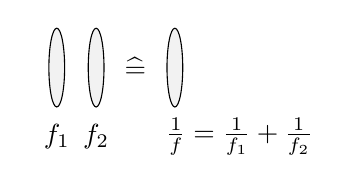
\begin{tikzpicture}
			\coordinate (1) at (-1,0);
			\coordinate (2) at (-.5,0);
			\coordinate (3) at (.5,0);
			\node at (0,0) {$ \widehat{=} $};
			\draw[fill=gray!10] (1) ellipse (.1cm and .5cm);
			\draw[fill=gray!10] (2) ellipse (.1cm and .5cm);
			\draw[fill=gray!10] (3) ellipse (.1cm and .5cm);
			\node[yshift=-25pt] at (1) {$ f_1 $};
			\node[yshift=-25pt] at (2) {$ f_2 $};
			\node[yshift=-25pt] at (3) {$\qquad \ \  \qquad \frac{1}{f} = \frac{1}{f_1} + \frac{1}{f_2} $};
		\end{tikzpicture}
	\end{minipage}%
	\\
	Berechnung:
	\begin{equation*}
	b_1 \ \tx{der 1ten Linsen} = \tx{virtuelle Gegenstandsweite} \ a_2 = b_1 - D \ \tx{der zweiten Linse}
	\end{equation*}
	\begin{itemize}
		\item[1.] Linse $ \frac{1}{a} + \frac{1}{b_1} = \frac{1}{f_1} $
		\item[2.] Linse $ -\frac{1}{b_1 - D} + \frac{1}{b} = \frac{1}{f_2} $
	\end{itemize}
	\begin{equation*}
	\Rightarrow \qquad \rmbox{\frac{1}{f} = \frac{1}{f_1} + \frac{1}{f_2}} \qquad \rmbox{D_{\tx{ges}} = D_1 + D_2}
	\end{equation*}
	\item \textbf{Fernrohr (Kepler): Abstand der Linsen $ = $ Summe der Brennweiten $ f_1 + f_2 $}\\
	\begin{minipage}{.5\linewidth}
		$ \Rightarrow $ Zwischenbild in der Brennebene\\[10pt]
		Sehwinkel vor Objektiv:
		\begin{equation*}
		\alpha \approx \frac{B}{f_1}
		\end{equation*}
		Sehwinkel nach Okular:
		\begin{equation*}
		\beta \approx \frac{B}{f_2}
		\end{equation*}
	\end{minipage}%
	\begin{minipage}{.5\linewidth}
		%t6:
		\centering
		\begin{tikzpicture}
		\coordinate (1) at (-2,0);
		\coordinate (2) at (1,0);
		\draw[fill=gray!10] (1) ellipse (.15cm and 1.3cm);
		\draw[fill=gray!10] (2) ellipse (.15cm and 1.3cm);
		\draw (-4,0) -- (2.5,0);
		\draw[dashed] ($ (1) + (0,-1.5) $) -- ++(0,3);
		\draw[dashed] ($ (2) + (0,-1.5) $) -- ++(0,3);
		\coordinate (B) at (0,-1);
		\draw[thick,->] (0,0) -- (B) node[left,yshift=15pt] {$ B $};
		\coordinate (1u) at ($ (1) + (0,.5) $);
		\coordinate (1d) at ($ (1) + (0,-1) $);
		\coordinate (2u) at ($ (2) + (0,.5) $);
		\coordinate (2d) at ($ (2) + (0,-1) $);
		\draw (1u) -- (B) -- (2u);
		\draw (1) -- (B) -- (2);
		\draw (1d) -- (B) -- (2d);
		\draw (1u) -- ++(157.5:1.5cm);
		\draw (1) -- ++(157.5:1.5cm);
		\draw (1d) -- ++(157.5:1.5cm);
		\draw (2u) -- ++(45:1.5cm);
		\draw (2) -- ++(45:1.5cm);
		\draw (2d) -- ++(45:1.5cm);
		\node[above] at (.5,0) {$ f_1 $};
		\node[above] at (-1,0) {$ f_2 $};
		\node[circle,fill=black,inner sep=1pt,minimum size=1pt] at (0,0) {};
		\node[circle,fill=black,inner sep=1pt,minimum size=1pt] at (2,0) {};
		\centerarc[thick,<->](-2,0)(180:157.5:1.25cm);
		\node[left,yshift=4pt,xshift=-15pt] at (-2,0) {$ \alpha $};
		\centerarc[thick,<->](1,0)(0:45.5:1.25cm);
		\node[right,yshift=7pt,xshift=15pt] at (1,0) {$ \beta $};
		\end{tikzpicture}
	\end{minipage}%
	\\
	$ \Rightarrow $ Vergrößerung $ V = \frac{\beta}{\alpha} = \frac{B}{f_2} \frac{f_1}{B} = \frac{f_1}{f_2} $\\[5pt]
	\emph{Bemerkung:}
	\begin{itemize}
		\item Kepler Fernrohr: Bild wird invertiert
		\item Galilei Fernrohr: Sammellinse und Zerstreuungslinse\\
		keine Invertierung und kürzere Bauweise
		\item Fernglas:\\
		\folie{Galilei Fernrohr und Fernrohr mit drei Linsen}
	\end{itemize}
	\item \textbf{Mikroskop: Abstand der Linsen $ \gg $ Summe der Brennweiten $ f_2 + f_1 $}\\
	Gegenstand nah am Objektiv
	% t7:
	\begin{center}
	\begin{tikzpicture}
		\coordinate (1) at (-3,0);
		\coordinate (2) at (1,0);
		\draw[fill=gray!10] (1) ellipse (.15cm and 1.3cm);
		\draw[fill=gray!10] (2) ellipse (.2cm and 1.8cm);
		\draw (-5,0) -- (3,0);
		\draw[dashed] ($ (1) + (0,-1.5) $) -- ++(0,3);
		\draw[dashed] ($ (2) + (0,-2) $) -- ++(0,4);
		\coordinate (ZB) at (0,-1);
		\coordinate (B) at ($ (2) + (1,1) $);
		\coordinate (G) at ($ (1) + (-1.5,.5) $);
		\draw[thick,->] (0,0) -- (ZB) node[left,yshift=15pt] {$ ZB $};
		\draw[thick,->] ($ (1) + (-1.5,0) $) -- (G) node[left,yshift=-8pt] {$ G $};
		\draw[thick,->] ($ (2) + (1,0) $) -- (B) node[right,yshift=-15pt] {$ B $};
		\coordinate (1u) at ($ (1) + (0,.5) $);
		\coordinate (1d) at ($ (1) + (0,-1) $);
		\coordinate (2u) at ($ (2) + (0,1) $);
		\coordinate (2d) at ($ (2) + (0,-1) $);
		\draw (G) -- (ZB) -- (B);
		\draw (G) -- (1u) -- (ZB) -- (2u) -- (B);
		\draw (G) -- (1d) -- (ZB) -- (2d) -- (B);
		\coordinate (f1) at ($ (1) + (1,0) $);
		\coordinate (f2) at ($ (1) + (-1,0) $);
		\coordinate (f3) at ($ (2) + (-.5,0) $);
		\coordinate (f4) at ($ (2) + (.5,0) $);
		\draw[thick] ($ (f1) + (45:.1) $) -- ++(-135:.2);
		\draw[thick] ($ (f1) + (-45:.1) $) -- ++(135:.2);
		\draw[thick] ($ (f2) + (45:.1) $) -- ++(-135:.2);
		\draw[thick] ($ (f2) + (-45:.1) $) -- ++(135:.2);
		\draw[thick] ($ (f3) + (45:.1) $) -- ++(-135:.2);
		\draw[thick] ($ (f3) + (-45:.1) $) -- ++(135:.2);
		\draw[thick] ($ (f4) + (45:.1) $) -- ++(-135:.2);
		\draw[thick] ($ (f4) + (-45:.1) $) -- ++(135:.2);
		\node[below,xshift=-5pt] at (f2) {$ f_1 $};
		\node[below,xshift=5pt] at (f4) {$ f_2 $};
		\node[yshift=-55pt] at (1) {$ \substack{\tx{1. Linse}\\\tx{Objektiv}} $};
		\node[yshift=-67.5pt] at (2) {$ \substack{\tx{2. Linse (Lupe)}\\\tx{Okular}} $};
	\end{tikzpicture}
	\end{center}
	\folie{anderes Bildschema Mikroskop} Veränderung durch Änderung der Tubuslänge\\
	Verstärkung durch Objektiv $ V_1 = \frac{B}{G} = \frac{b}{f_1} $\\
	Verstärkung durch Okular $ V_2 = \frac{25 \, \tx{cm}}{f_2} $\\
	$ \Rightarrow $ Vergrößerung: $$ V = V_1 V_2 = \frac{t \cdot 25 \, \tx{cm}}{f_1 f_2} $$
	$ t \approx 18 \, \tx{cm} $ wurde so definiert um den Vergleich von Geräten zu vereinfachen.
\end{enumerate}

% Vorlesung 7.11.18 (8)

\section{Elektronenoptik}

\folie{Elektronen Strahl}\\
\lcom{Die Idee hier ist das man einen Elektronenstrahl der von einem $\vec{E}$-Feld abgelenkt wird als wie eine optische Beugung betrachten...}\\
Elektronenstrahl Ablenkung durch elektrische und magnetische Felder

$$\vec{F} = q \vec{E}$$
$$\vec{F} = q (\vec{v} \times \vec{B})$$

\subsection{Beispiel: Brechungsgesetz für Elektronen}

$$\sin \alpha = \frac{v_{1,x}}{v_1} \qquad \sin \beta = \frac{v_{2,x}}{v_2}$$
el. Feld entlang $x$
$$v_{1,x} = v_{2,x}$$
$$\Rightarrow v_1 \sin \alpha = v_2 \sin \beta$$
\textbf{Definition}
$$\frac{n_2}{n_1} = \frac{v_2}{v_1}$$
Energieerhaltung
$$\frac{1}{2} mv^2_2 = \frac{1}{2} mv_1^2 + eU$$
$$v_1 = \sqrt{\frac{2eU_0}{m}}, \quad v_2 = \sqrt{\frac{2e(U+U_0)}{m}}$$
\frbox{$\Rightarrow$ Brechindex}{$$\frac{n_2}{n_1} = \sqrt{1 + \frac{U}{U_0}}$$}

\subsection{Elektrische Rohrlinse}

\subsection{Magnetische Linsen}

Lange Spule = homogenes Magnetfeld\\
Lorenz Kraft $\Rightarrow$ Spiralbahnen der Elektronen $\Rightarrow$ Bild wird gedreht\\
$\Rightarrow$ kleine Spule = inhomogene Magnetfelder $\Rightarrow$ Brechkraft \\
\folie{Elektronen in Magnetfeldern}
\subsection{Elektronenmikroskope}

\folie{Elektronmikroskop}\\
\lcom{Man kann ein Material untersuchen in dem man die Streuelektronen analysiert, die bei dem Elektronenmikroskop entstehen.}\\[5pt]
\lcom{Bei der SRT muss man nach Gedankenfehler suchen, bei Optik müssen wir die Näherungen als Fehlerquelle anschauen, ,,ZahnmedizinerInnen`` würden alle Fehlerpunkte auswendig gelernt haben, während ein Physiker überlegen ''ok, wir haben die geometrische Optik angewandt also alles was da schief gehen kann und so weiter.''}